\section{Attribute grammars}

The syntax directed translators use functions applied to the syntax tree to compute some semantic attributes.
In other words, they express the meaning of the sentence. 

Attribute grammars have the same expressive power as the Turing machine. 

Compilation is organized in two phases: 
\begin{enumerate}
    \item \textit{Lexical and syntactical analysis}, that produces the syntax tree. 
    \item \textit{Semantic analysis}, that produces the decorated syntax tree. 
        This phase is done using attribute grammars. 
\end{enumerate}

For simplicity the attribute grammar is defined with respect to an abstract syntax, that is a grammar that may be simpler than the real one, often ambiguous, but convenient. 
The ambiguity of the abstract syntax does not prevent a single-valued translation: the parser will pass to the semantic evaluator only one syntax tree. 

\paragraph*{Attribute grammar}
An attribute grammar is defined as follows: 
\begin{enumerate}
    \item A context-free syntax $G = \left( V, \Sigma, P, S \right)$ where $V$ and $\Sigma$ represent the terminal and nonterminal sets, $P$ comprises the production rule set, and $S$ serves as the axiom. 
        It is advisable (though not mandatory) to exclude the axiom from any rule RP.
    \item A collection of symbols, known as (semantic) attributes, is linked with both nonterminal and terminal syntax symbols. 
        The set of attributes associated with a symbol $\bigoplus$ is represented as $\text{attr}\left( \bigoplus \right)$.
        Within the grammar, the attribute set is divided into two distinct sets: the left and right attributes.
    \item A set of semantic functions (or rules) is defined with the following characteristics:
        \begin{itemize}
            \item Each function is linked to a production rule:
                  \[ p: D_0 \rightarrow D_1 D_2 \ldots D_r \quad r \geq 0\]
                  where $D_0$ is a nonterminal, and the other symbols can be either terminal or nonterminal.
            \item The production $p$ is referred to as the syntactic support of the function and may be shared among different functions.
            \item The attribute $\sigma$ associated with a symbol $D_k$ is denoted by $\sigma_k$ or $\sigma_D$ if the syntactic symbol occurs exactly once in production $p$.
            \item A semantic function is structured as follows:
                  \[ \sigma_k := f \left( \text{attr} \left( \left\{ D_0, D_1, \ldots , D_k \right\} \right) \setminus \left\{ \sigma_k \right\}\right) \quad 0 \leq k \leq r \]
                  where function $f$ assigns the computed value to the attribute $\sigma$ of symbol $D_k$, and its arguments can include any attributes of the same production $p$, excluding $\sigma_k$ itself.
            \item Generally, semantic functions cover their entire domain and are expressed in a suitable notation, termed semantic metalanguages, which can be informal.
            \item A function $\sigma_0 := f(\ldots)$ defines an attribute, identified as left, of the nonterminal $D_0$, which serves as the LP (or parent) of the production.
            \item A function $\sigma_k := f(\ldots), \ k \geq 1$ defines an attribute, labeled as right, of a symbol (sibling or child) $D_k$ present in the RP.
            \item The same attribute cannot serve as left in one function and right in another.
            \item Since terminal characters never appear in the left part, their attributes cannot be of the left type.
        \end{itemize}
    \item The set $\text{fun}(p)$ of functions supported by production $p$ must adhere to the following conditions:
        \begin{enumerate}
            \item For each left attribute $\sigma_0$ of $D_0$, there must exist exactly one function in $\text{fun}(p)$ defining the attribute.
            \item No function within $\text{fun}(p)$ defining the attribute exists for each right attribute $\delta_0$ of $D_0$.
            \item No function within $\text{fun}(p)$ defining the attribute exists for each left attribute $\sigma_i, i \geq 1$.
            \item For each attribute $\delta_i, i \geq 1$, there must exist exactly one function in $\text{fun}(p)$ defining the attribute.
        \end{enumerate}
        The left attributes $\sigma_0$ and the right ones $\delta_i$ with $i \geq 1$ are termed internal for production $p$ because functions supported by $p$ define them. 
        Conversely, the right attributes $\delta_0$ and left attributes $\sigma_i$ with $i \geq 1$ are termed external for production $p$ since functions supported by other productions define them.    
    \item Certain attributes can be initialized with constant values or values computed by external functions. 
        This is frequently observed in the case of lexical attributes, which are linked to terminal symbols. 
        In such instances, the grammar does not stipulate a specific computation rule.
\end{enumerate}
Semantic function are applied following the dependencies among attributes starting from attributes whose value is known. 
Often the initial values are in the leaves, possibly precomputed by the lexical analysis. 

The attributes of an attribute grammar can be of two different types: 
\begin{itemize}
    \item \textit{Left attribute} (or synthesized): the semantic function $\sigma_0=f(\dots)$, whereby the attribute $\sigma_0$ is assigned a value, in a rule where $\sigma_0$ is an attribute of the left nonterminal of the rule. 
    \item \textit{Right attribute} (or inherited):  the semantic function $\delta_i=f(\dots), i \geq 1$, whereby attribute $\delta_i$ is assigned a value, in a rule where $\delta_i$ is an attribute of a symbol in the right rule part. 
\end{itemize}

\subsection{Dependence graph}
The dependence graph $dep_p$ for the attributes associated with a syntax rule $p$ is a directed graph where: 
\begin{itemize}
    \item The nodes are the attributes. 
    \item There is an arc from every argument to the result. 
    \item Left attributes placed to the left of three node and right ones to the right. 
\end{itemize}

A grammar is termed loop-free if the dependence graph of the tree is acyclic for every sentence.

Under the acyclicity condition, the equations can be ordered so that each semantic function is applied after the functions that compute its arguments. 
This results in a value for the solution, given the totality of the functions. 
The solution is unique, similar to a system of linear equations. 
The topological ordering method can be used to provide a total order of nodes, although this is an inefficient way to compute the solution. 
It would require applying the sorting algorithm even before computing the attribute values.

Checking whether a given grammar is acyclic poses another problem. 
Since the source language is typically infinite, exhaustive enumeration of all trees for the acyclicity test is impractical. 
An algorithm determining if an attribute grammar is acyclic exists but is $\mathcal{NP}$-complete and thus not used in practice. 
It is more convenient to test certain sufficient conditions.

\subsection{One-sweep semantic evaluation}
An efficient evaluator should be capable of computing all attributes of a tree in just one pass. 
This involves traversing the tree through a depth-first search, allowing for attribute evaluation in a single sweep across the entire tree.

Let $N$ represent a node in the tree, with $N_1, \dots, N_r$ as its children, and $t_i$ denoting the subtree rooted at node $N_i$.
A depth-first algorithm starts by visiting the tree root, and to visit the subtree $t_N$ rooted at node $N$, it recursively follows these steps:
\begin{enumerate}
    \item Conduct a depth-first visit of the subtrees $t_1, \ldots, t_r$ in an order corresponding to a permutation  of $1, \ldots, r$. 
    \item Evaluate the attributes with the following principles:
        \begin{itemize}
            \item Before entering and evaluating a subtree $t_N$, compute the right attributes of node $N$  (the root of the subtree). 
                These attributes are then passed as input parameters to the procedure implementing the visit.
                Procedure calls with input parameter passing constitute the "descending phase" of the visit.
            \item At the end of the visit of subtree $t_N$, compute the left attributes of node $N$. 
                These attributes are the output parameters of the procedure implementing the visit.
                Procedure returns with output parameter passing constitute the "ascending phase" of the visit.
          \end{itemize}
\end{enumerate}
Not all grammars are compatible with this one-sweep procedure because more intricate functional dependencies may necessitate multiple visits to the same node.
\begin{figure}
  \centering
  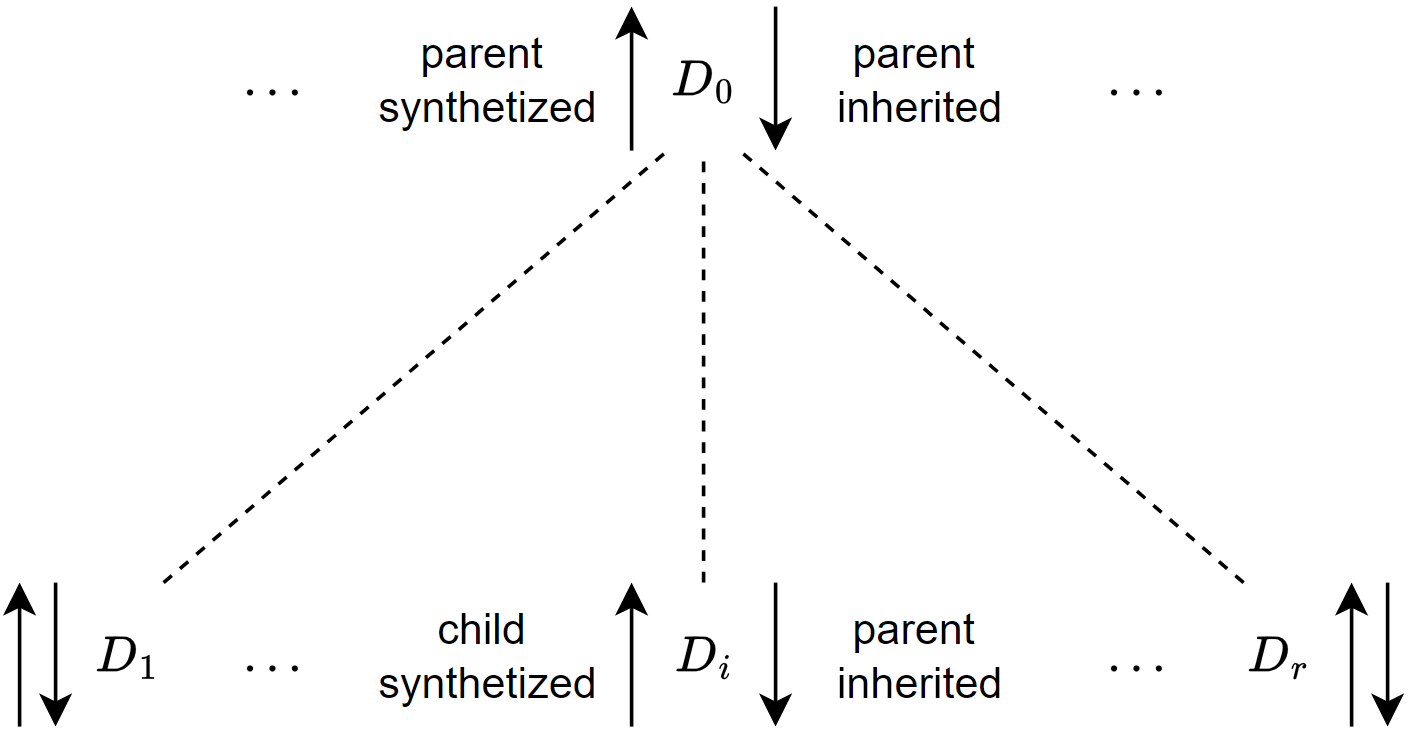
\includegraphics[width=0.5\linewidth]{images/sweep.png}
  \caption{One-sweep semantic evaluation}
\end{figure}


\paragraph*{One-Sweep Grammar}
For each production $p: D_0 \rightarrow D_1 D_2 \ldots D_r$ with $r \geq 0$, it is necessary to introduce a new relation between the symbols in the right part of the production.
This allows the creation of a directed graph, referred to as the sibling graph $\text{sibl}_p$, which captures the relations between the symbols in the right part of the production $p$.
The nodes of $\text{sibl}_p$ are the symbols $\left\{ D_1, \ldots , D_r \right\}$ of the production, and has arcs $D_i \rightarrow D_j$, with $i \neq j, \ i,j \geq 1$ if in the dependence graph $\text{dep}_p$ there is an arc $\sigma_i \rightarrow \delta_j$ from an attribute of symbol $D_i$ to an attribute of symbol $D_j$.
Note that the nodes in the sibling graph are syntactical symbols, distinct from the attributes in the dependence graph.

A grammar satisfies the one-sweep condition if, for each production $p : D_0 \rightarrow D_1 D_2 \ldots D_r,  r \geq 0$ that has a dependence graph $\text{dep}_p$, the following clauses hold at the same time:
\begin{enumerate}
    \item Graph $\text{dep}_p$ contains no circuit (is acyclic).
    \item Graph $\text{dep}_p$ does not contain a path $\lambda_i \rightarrow \ldots \rightarrow \rho_i, \ i \geq 1$ that goes from a left attribute $\lambda_i$ to a right attribute $\rho_i$ of the same symbol $D_i$, where $D_i$ is a sibling of $D_0$.
    \item Graph $\text{dep}_p$ contains no arc $\lambda_0 \rightarrow \rho_i, \ \geq 1$, from a left attribute of the father node $D_0$ to a right attribute of a sibling node $D_i$.
    \item The sibling graph $\text{sibl}_p$ contains no circuit (is acyclic).
\end{enumerate}

\paragraph*{Construction of the one-sweep evaluator}
The procedure visits the subtrees, computes, and returns the left attributes of the root of the subtree.
For each production $p : D_0 \rightarrow D_1 D_2 \ldots D_r, \ r \geq 0$:
\begin{enumerate}
    \item Choose a topological order (TOS) of the nonterminals $D_1, D_2, \ldots  D_r$ with respect to the sibling graph $\text{sibl}_p$.
    \item For each symbol $D_i,  1 \leq i \leq r$, choose a topological order (TOR) of the right attributes of symbol $D_i$ with respect to the dependence graph $\text{dep}_p$.
    \item Choose a topological order (TOL) of the left attributes of symbol $D_0$ with respect to the dependence graph $\text{dep}_p$.
\end{enumerate}
The three orders TOS, TOR and TOL prescribe how to arrange the instructions of the procedure that implements the visit of the subtree $t_N$.

\subsection{Combined syntax and semantic analysis}
The integration of syntax tree construction and attribute computation allows the parser to handle both responsibilities, invoking semantic functions as needed. 
In this context, we assume the use of a pure BNF grammar, avoiding the complexity that EBNF productions would introduce in specifying the relationship between syntax symbols and attributes.
\begin{table}[H]
    \centering
    \begin{tabular}{c|c|c}
        \textbf{Source language}  &                                                   & \textbf{Tool}         \\ \hline
        regular                   & lexical analysis with lexical attributes          & flex, lex             \\
        LL(k)                     & recursive descent parser with attributes          &                       \\
        LR(k)                     & shift-reduce parser with attributes               & yacc, bison
    \end{tabular}
    \caption{Combined syntax and semantic}
\end{table}

\paragraph*{Lexical analysis with attribute evaluation}
The lexical analyzer, or scanner, not only divides the source text into lexemes (or tokens) but also assigns semantic attributes to these lexemes. 
Lexemes, representing the smallest meaningful substrings, are categorized into lexical classes defined by regular formal languages, such as regular expressions or sets of strings. 
The lexical and syntactic specifications operate at different levels, with the lexical level determining the form of lexemes and the syntactic level assuming these lexemes as terminal symbols in the grammar.
Some lexemes may carry additional meaning, serving as semantic attributes computed by the lexical analyzer.

\paragraph*{Attributed recursive descent translator}
In cases where a syntax is suitable for deterministic top-down parsing, attribute evaluation can proceed during parsing, provided that the functional dependencies of the grammar satisfy conditions beyond those of a one-sweep grammar. 
The one-sweep algorithm traverses the syntax tree in a depth-first order, which may differ from the natural order constructed by a top-down parser. 
To merge these two procedures, functional dependencies must be free from any conflicts that might result from differing tree traversal orders.

\paragraph*{L-condition}
A grammar satisfies the condition L if, for each production $p: D_0 \rightarrow D_1 \ldots D_r$, it holds:
\begin{enumerate}
    \item The one-sweep condition is satisfied. 
    \item The sibling graph $\text{sibl}_p$ contains arc $D_j \rightarrow D_i, j > i \geq 1$.
\end{enumerate}
The second condition in the L-condition prevents a right attribute of node $D_i$ from depending on any attribute of a node $D_j$ placed to its right in the production $p$.

\paragraph*{Attribute grammar and deterministic parsing}
Consider an attribute grammar $G$, where:
\begin{itemize}
    \item The syntax satisfies the $LL(k)$ condition.
    \item The semantic rules satisfy the L-condition.
\end{itemize}
It's possible to construct a top-down deterministic parser with attribute evaluation able to compute the attributes of $G$ at parsing time.